%%%%%%%%%%%%%%%%%%%%%%% file template.tex %%%%%%%%%%%%%%%%%%%%%%%%%
%
% This is a general template file for the LaTeX package SVJour3
% for Springer journals.          Springer Heidelberg 2010/09/16
%
% Copy it to a new file with a new name and use it as the basis
% for your article. Delete % signs as needed.
%
% This template includes a few options for different layouts and
% content for various journals. Please consult a previous issue of
% your journal as needed.
%
%%%%%%%%%%%%%%%%%%%%%%%%%%%%%%%%%%%%%%%%%%%%%%%%%%%%%%%%%%%%%%%%%%%
%
% First comes an example EPS file -- just ignore it and
% proceed on the \documentclass line
% your LaTeX will extract the file if required
\begin{filecontents*}{example.eps}
%!PS-Adobe-3.0 EPSF-3.0
%%BoundingBox: 19 19 221 221
%%CreationDate: Mon Sep 29 1997
%%Creator: programmed by hand (JK)
%%EndComments
gsave
newpath
  20 20 moveto
  20 220 lineto
  220 220 lineto
  220 20 lineto
closepath
2 setlinewidth
gsave
  .4 setgray fill
grestore
stroke
grestore
\end{filecontents*}
%
\RequirePackage{fix-cm}
%
%\documentclass{svjour3}                     % onecolumn (standard format)
%\documentclass[smallcondensed]{svjour3}     % onecolumn (ditto)
\documentclass[smallextended, natbib]{svjour3}       % onecolumn (second format)
%\documentclass[twocolumn]{svjour3}          % twocolumn
%
\smartqed  % flush right qed marks, e.g. at end of proof
%

\usepackage{graphicx}
\usepackage{amsmath}
\usepackage{algorithm}
\usepackage{algorithmic}
\usepackage{tikz}
\renewcommand{\algorithmicrequire}{\textbf{Initialize:}}

\usepackage{verbatim} %TODO delete before submission
%\usepackage[numbers]{natbib}%TODO delete before submission

%TODO Zitierweise ändern, sieht schrecklich aus
%
% \usepackage{mathptmx}      % use Times fonts if available on your TeX system
%
% insert here the call for the packages your document requires
%\usepackage{latexsym}
% etc.
%
% please place your own definitions here and don't use \def but
% \newcommand{}{}
%
% Insert the name of "your journal" with
% \journalname{myjournal}
%
\begin{document}

\title{Application of Reinforcement Learning Methods
%\thanks{Grants or other notes
%about the article that should go on the front page should be
%placed here. General acknowledgments should be placed at the end of the article.}
}
\subtitle{Group 19 - Final Project Report}

%\titlerunning{Short form of title}        % if too long for running head

\author{Yannik P. Frisch \and Tabea A. Wilke \and Maximilian A. Gehrke %etc.
}

\institute{Maximilian A. Gehrke \at
	TU Darmstadt, Germany\\
	\email{maximilian\_alexander.gehrke@stud.tu-darmstadt.de}           %  \\
	%             \emph{Present address:} of F. Author  %  if needed
	\and
	Yannik P. Frisch \at
	TU Darmstadt, Germany\\
	\email{yannik\_phil.frisch@stud.tu-darmstadt.de}
	\and
	Tabea A. Wilke \at
	TU Darmstadt, Germany\\
	\email{tabeaalina.wilke@stud.tu-darmstadt.de}
}

\maketitle

\section{Introduction}
\label{sec:intro}
We shortly present two state-of the art reinforcement learning algorithms, the 
\textit{Deep Deterministic Policy Gradient} and the \textit{Natural Actor 
Critic}. Both algorithms are evaluated on the simulated Quanser Robots 
platforms \textit{BallBalancerSim-v0}, \textit{CartPoleStabShort-v0} and 
\textit{Qube-v0}. We furthermore present the results of training both 
algorithms on the \textit{BallBalancerSim-v0} and evaluating it on the pyhiscal 
\textit{BallBalancerRR-v0} platform. Finally, we close with a discussion of the 
results.
\newpage
\section{Deep Deterministic Policy Gradient}
\label{sec:ddpg}
The \textit{Deep Deterministic Policy Gradient} approach 
\citep{lillicrap2015continuous} is an application of the \textit{Deep 
Q-Learning} algorithm \citep{mnih2013playing} to actor-critic methods 
\citep{konda2000actor} in combination with the \textit{Deterministic Policy 
Gradient} \citep{silver2014deterministic}. It is a model-free and off-policy 
algorithm, learning a deterministic policy. We separated the learning process 
completely from the algorithm's other components. The critic is updated using 
the temporal difference error. It is calculated from using the target networks 
which are constrained to slow changes with rate $\tau$ to improve the stability 
of learning. The actor is trained by using the integrated update rule from 
\cite{lillicrap2015continuous} as it's loss function. Both networks are 
addressed and can be modified in a separate file, same as the replay buffer, 
which is used to sample independently and identically distributed mini-batches, 
randomly selected to temporarily decorrelate them. The action noise to ensure 
exploration was also kept completely independent from the training algorithm as 
intended by \citep{lillicrap2015continuous} and is just added to the output of 
the actor. We clip this output to ensure it suits the environment.

\subsection{Evaluation on BallBalancerSim-v0}
The Quanser Robots \textit{BallBalancerSim-v0} environment consist of a plate whose angles can be controlled by the input actions. The goal is to balance a ball on the plate, receiving a maximum reward of 1.0 per time-step for balancing it in the middle of the plate. The environment ends after a maximum of 1000 time-steps.

We started our evaluations with using two hidden layers with 100 and 300 hidden neurons for the actor and the critic networks and their targets. The learning rates are set to $\alpha_{actor}=1e-4$ and $\alpha_{critic}=1e-3$.  In the left row of figure \ref{ddpg:ball} one can find our first acceptable results. Discounting is set to $\gamma=0.99$, we did soft target updates with $\tau=1e-4$, used a mini-batch size of 64 and a total replay buffer size of 1e6. We slightly increased the noise to $\sigma_{OU}=0.2$ and $\theta_{OU}=0.25$ as the environments action space has an higher amplitude compared to the \textit{Pendulum-v0} trained on in \citep{lillicrap2015continuous}.

The algorithm did learn to balance the ball, but was not very stable, which can also be read from the learning progress plot. To further increase the stability, we increased th mini-batch size used to sample from the replay buffer, and reduced the noise again. Using weight regularization did not seem to be helpful, so we set it to zero.

Figure \ref{ddpg:ball:gamma} shows the training process where discounting is set to $\gamma=0.2$ compared to $\gamma=0.99$. One can see discounting is crucial to solve this environment.

\begin{figure}
	\centering
	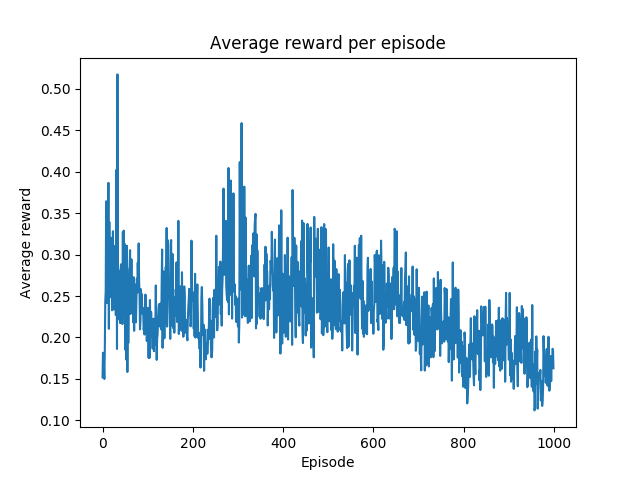
\includegraphics[width=0.4\textwidth]{plots/ddpg_ball_low_gamma.png}
	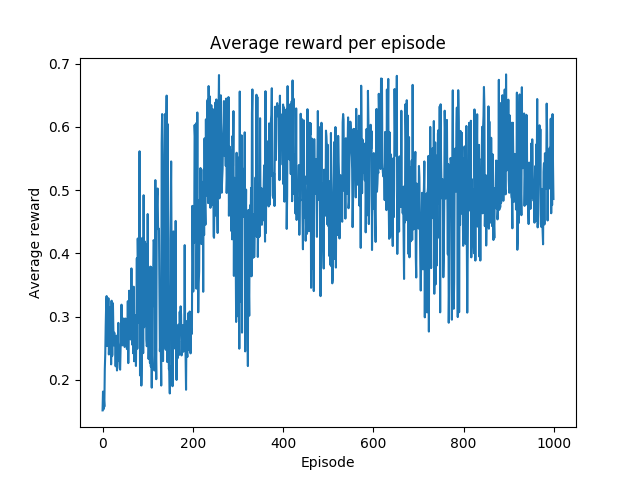
\includegraphics[width=0.4\textwidth]{plots/ddpg_ball_high_gamma.png}
	\caption{The left figure shows the cumulative reward per episode during the training process with $\gamma$ set to 0.2. The right one displays the process for $\gamma=0.99$. Using discounting close to 1 was very important.}
	\label{ddpg:ball:gamma}
\end{figure}
We tried to reduce the computational effort by only using a single hidden layer with 100 hidden neurons instead of two layers. The impact on the performance is shown in the middle row of figure \ref{ddpg:ball}. The learning suffered from instabilities, so we decided to weight the stability of using two hidden layers higher than the performance loss.

Our best results can be found in the right row of figure \ref{ddpg:ball} where we set the OU action noise equal to the one used in the original paper with $\sigma_{OU}=0.15$ and $\theta_{OU}=0.2$. We used slightly harder updates with $\tau=1e-3$, and achieved an average cumulative reward of about 650 for 25 episodes of evaluation. The learning process took about 3 hours for 1000 episodes. Further evaluations are needed to improve the training even more.

\begin{figure}
	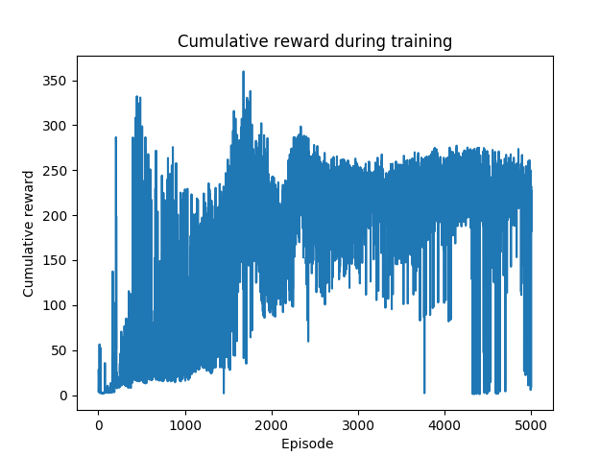
\includegraphics[width=0.325\textwidth]{plots/ddpg_ball_first_train.png}
	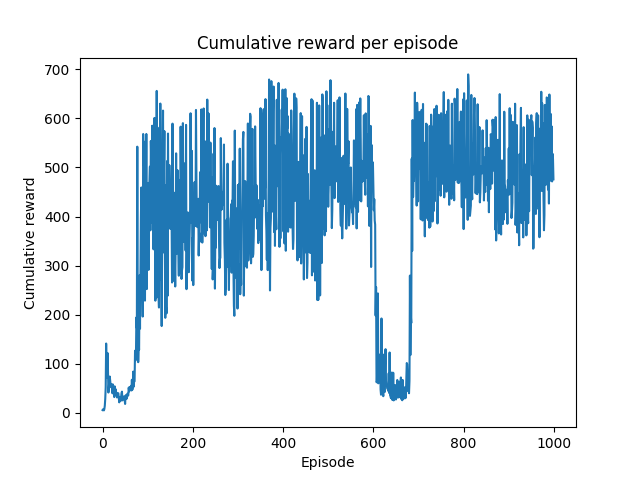
\includegraphics[width=0.325\textwidth]{plots/ddpg_ball_1layer_train.png}
	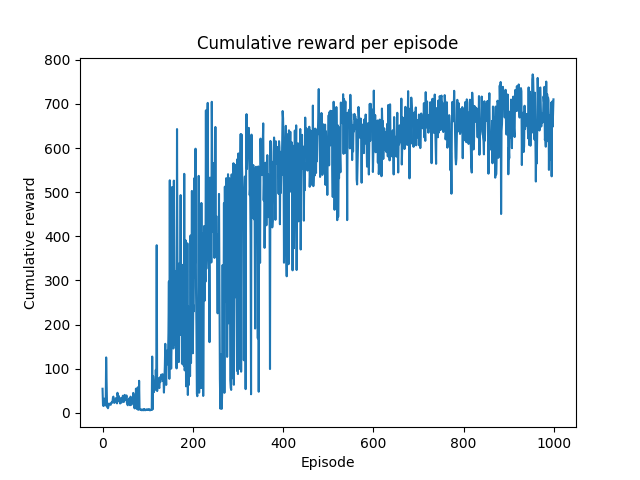
\includegraphics[width=0.325\textwidth]{plots/ddpg_ball_best_train.png}
	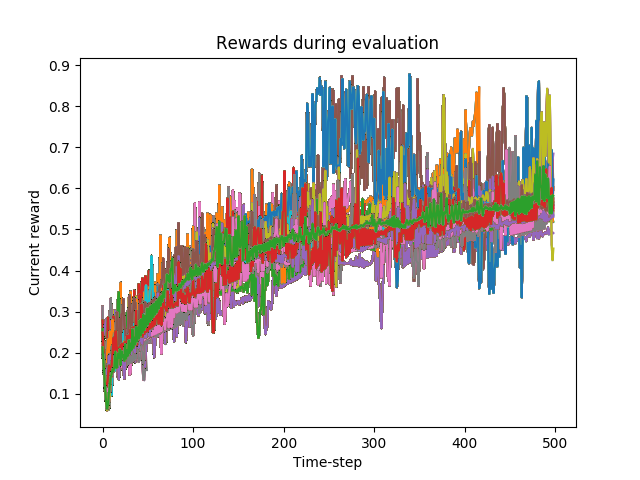
\includegraphics[width=0.325\textwidth]{plots/ddpg_ball_first_eval.png}
	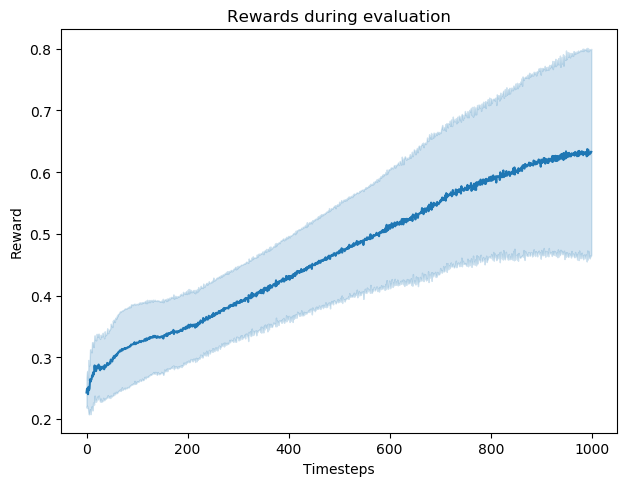
\includegraphics[width=0.295\textwidth]{plots/DDPGballbalancer24-2-16.png}
	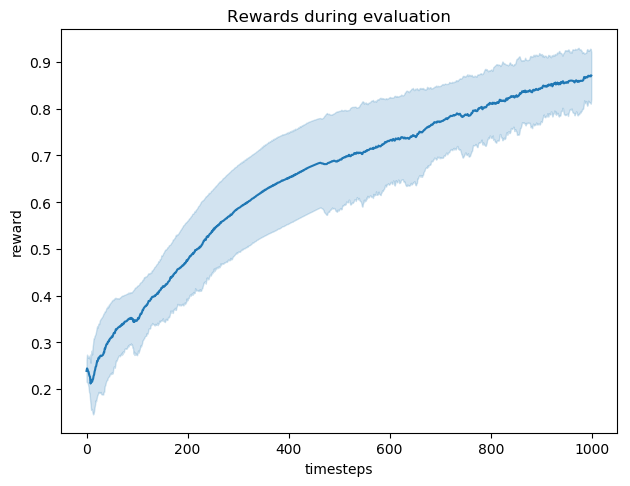
\includegraphics[width=0.295\textwidth]{plots/DDPGballbalancer26-2-20.png}

	\caption{The figure displays the training process in the first row and the evaluation results in the second row. Early learning successes can be found in the left column, while the middle column shows the influence of using only a single hidden layer. The right column gives the plots of our best training result.[EDIT: ALIGN PLOTS + LEFT PLOT IS WRONG (WRONG ENV...)]}
	\label{ddpg:ball}
\end{figure}

\subsection{Evaluation on CartPoleStabShort-v0}
The Quanser Robots \textit{CartPoleStabShort-v0} environment consists of a movable car with a singular pendulum attached. The car can be controlled by input actions. The goal is to balance the pendulum, starting from a vertical position and the reward is depending on the angle, with a maximum of 2.0 per time-step for balancing the pendulum straight upright.

We achieved some progress using [x]. The results are displayed in [x].

\subsection{Evaluation on Qube-v0}
The Quanser Robots \textit{Qube-v0} environment implements the Furuta Pendulum, which consists of a motor controlling one horizontal arm. One end of the joint is attached to the motor, the other end is attached to another vertical arm, which can only be controlled indirectly by controlling the first arm. More details about the Furuta Pendulum can be found in our paper about it.

The goal is to balance the second arm in upright position, receiving a maximum reward of 0.02 per time-step. The environment stops after 300 time-steps. We did not get any useful results re-using the parameters we found for \textit{BallBalancer-v0}. Using an Ornstein Uhlenbeck similar to the one used in citep{lillicrap2015continuous}, did not seem to help to deal with the local optima of the environment. Setting the randomness $\sigma_{OU}$ too small resulted in too less exploration. Choosing a higher $\sigma_{OU}$ resulted in better exploration but much less stability. Examples are displayed in figure \ref{ddpg:qube}.

No stable training process could be achieved. To address this issue we started using a consistent gaussian noise. Unfortunately this did also not help the training process, and seemed to be even more unstable. Figure \ref{ddpg:qube} shows a result of using gaussian noise in the right plot. The algorithm seemed to learn well for a period of time, but tended to overwrite these progress. Lowering the target update rate $\tau$ did not help, nether did lowering the actor and critic learning rates.

\begin{figure}
	\begin{center}
	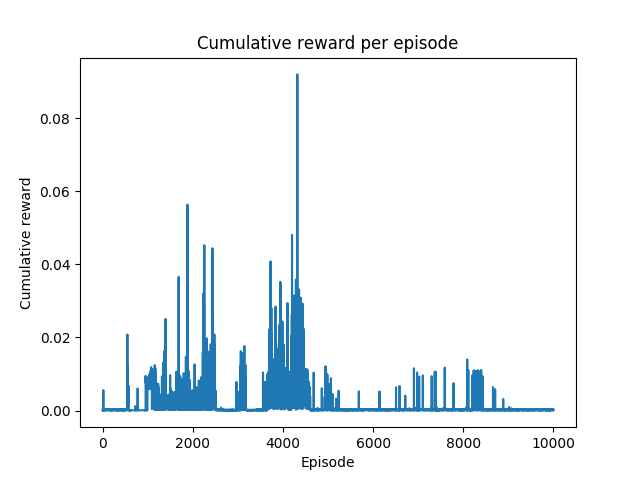
\includegraphics[width=0.325\textwidth]{plots/ddpg_qube_ou_bad_train.png}
	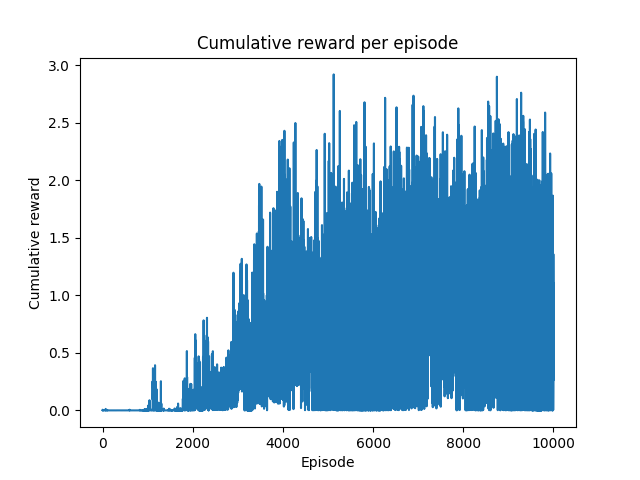
\includegraphics[width=0.325\textwidth]{plots/ddpg_qube_ou_better_train.png}
	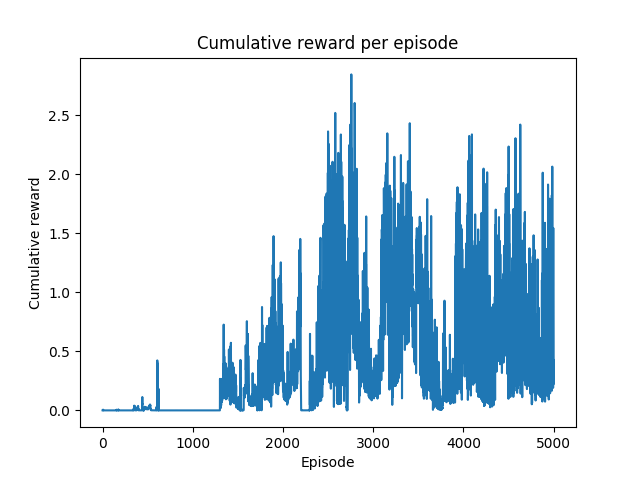
\includegraphics[width=0.325\textwidth]{plots/ddpg_qube_gauss.png}
	\caption{Assuming the parameters from our best result on \textit{BallBalancerSim-v0}, we achieved the performance shown in the left plot on \textit{Qube-v0}. The middle plot shows the changes when using more OU noise, i.e. $\sigma=3.2$. The right plot displays the result of training with a gaussian noise with mean zero and 
	standard deviation $\sigma=0.7$. The mini-batch size was also increased to 
	256.}
	\label{ddpg:qube}
	\end{center}
\end{figure}

Our experiments induced several things: Using a higher batch size seemed to increase the stability to a certain level, but also highly increased the computational effort. 256 seemed to be a good batch-size. The decisions harder or softer updates, controlled by $\tau$, and the amount of action noise for exploration seemed to be very important but also very hard to tune. E.g. choosing $\tau=1e-2$ resulted in an agent tending to overwrite what he already learned, while setting $\tau=1e-4$ prevented him from learning anything. So we chose $\tau=1e-3$, but this alone was not sufficient for effective learning. Reducing the action noise added to the actor output did also not help. Further evaluations are needed to find the right set of hyper-parameters for this environment. 

% ----- NAC ----- %

\section{Natural Actor Critic}
\label{sec:nac}

The \textit{Natural Actor Critic (NAC)} \citep{peters2008natural} is a model-free, off-policy algorithm, which learns the optimal policy of a reinforcement learning problem by applying the natural gradient \citep{amari1998natural} on an actor-critic approach \citep{sutton1998introduction}. We implemented the episodic NAC \citep{peters2008natural} which takes a fixed number of steps (equals one or more trajectories) in the environment before applying updates to the actor and critic. The actor is an approximation of the policy and the critic is an approximation of the value function. We implemented both, the actor and the critic, by using neural networks in tensorflow.

\subsection{The Critic Network}
For the critic, we introduced a neural network with a single hidden layer. The input layer equals the state dimension of the environment. It is fully connected to the hidden layer, which again is fully connected to a single output node and uses a ReLu activation function \citep{glorot2011deep}. 

To train the network, we calculate the discounted return for all states we visited since the last update and compare it to the discounted return approximation of the critic. Then, we take the least squares error between the two arrays as loss and minimize it by applying an Adam optimizer \citep{kingma2014adam}.

\textit{Parameters:} We used a hidden layer with 10 nodes and a learning rate of 0.1 for all environments. We tried to add more hidden nodes and experimented with the learning rate, but could not depict any significant improvements.

\subsection{The Actor Network}

The actor network has an input and an output layer, which are fully connected, and uses a softmax activation function. The input layer matches the dimension of the state, the output layer matches the dimension of the action space. If we feed an observation to the network, the output is an array of probabilities for each action. To select which action to take, we stochastically sample an action w.r.t these probabilities.

To train the network, we use the critic to calculate the advantages for all states we visited since the last update. Then we feed the advantages, states and actions to the actor and update the actors parameters with the natural gradient. For this, we compute the cost function, it's gradient w.r.t the actor network parameters and the inverse of the Fisher information matrix. To get the inverse, we apply singular value decomposition \citep{golub1965calculating}.

\textit{Parameters}: We trained all of the environments without a hidden layer and with a learning rate of 0.001. We tried to add a hidden layer and change the learning rate, but did not get any improved results.

\subsection{Evaluation on the BallBalancerSim-v0}

The NAC algorithm learned to solve the ball balancer extremely well. Already with 300 updates and 2000 steps per update, the ball balancer manages to hold the ball on the platform and navigate it slowly into the middle. The more steps the environment was allowed to do between updates, the greater became the cumulative reward. Our best run was a simulation with 1000 updates, 7000 steps per update and a discount factor of 1. This returned an cumulative average trajectory reward of 600.53. We believe that we would get an even higher average cumulative trajectory reward with more steps per update. 

The number of updates was not as important as the number of steps between updates. Figure \ref{fig:nac} shows in the top left corner that already after 300 steps we reached trajectories with cumulative rewards of 600. From this point onwards, the longer we update the more stable the algorithm gets (less trajectories with cumulative rewards under 600), but the average trajectory reward does not improve anymore.

Further, we can see in the bottom left corner of figure \ref{fig:nac} that even for our best run, the average reward per time step increased very slowly. This reflects the behavior of the environment, which moves the ball very slowly to the middle, where the environment returns increased rewards. Our idea was to apply a basis function to the rewards which pulls the high rewards from the low rewards even further, but did not have any success with it's implementation.

\subsection{Evaluation on CartPoleStabShort-v0 and CartPoleStabLong-v0}

We managed to get a nearly perfect result for the cart pole balancing task. Our best model depicts an average cumulative trajectory reward of 19768.60, which is slightly less than the possibly maximum of 20000. We used 300 updates with 2000 steps and a discount factor of 0.99 to achieve these results. However, the algorithm does not always learn this perfectly. Most of the times, the algorithm manages to balance the pole, but does not manage to hold the cart in the middle. 

Figure \ref{fig:nac} shows for a configuration of 300 updates, 2000 steps per update and a discount factor of 0.99  at the top mid that the algorithms learns fast and at the bottom mid that each time step gets a good reward. The problem is that the trajectories end after approximately 1000 steps.

As an additional task, we also evaluated NAC on the cart pole balancing task with a long pole. We used 300 updates with 200 steps, a discount factor of 0.99 and achieved an average cumulative trajectory reward of 18800.84.

\begin{figure}
	\begin{center}
		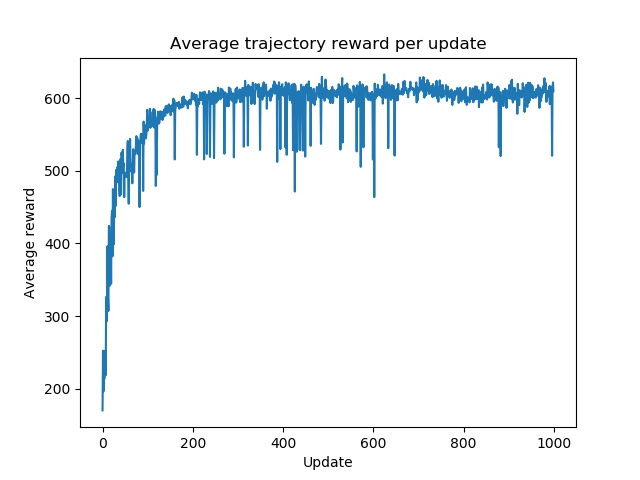
\includegraphics[width=0.325\textwidth]{plots/NAC_BB_training_mean_600.png}
		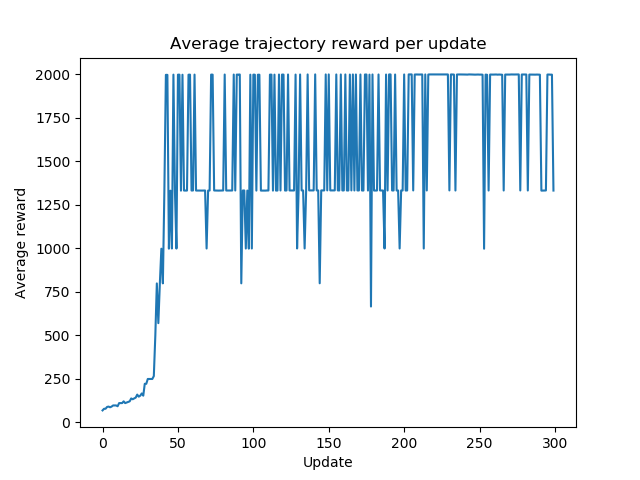
\includegraphics[width=0.325\textwidth]{plots/NAC_CP_mean_traj_update_reward.png}
		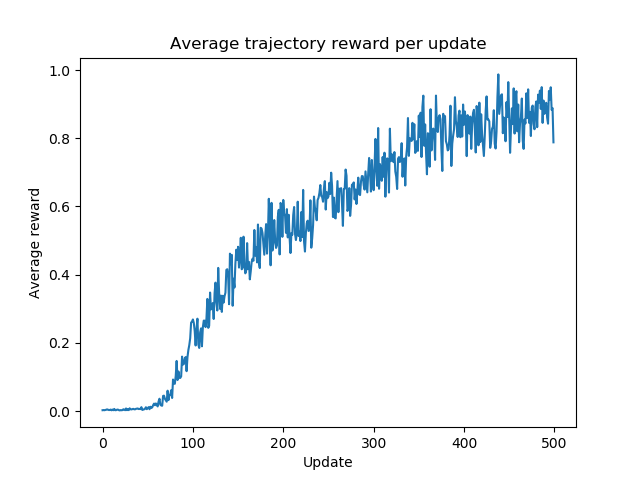
\includegraphics[width=0.325\textwidth]{plots/NAC_Qube_mean_traj_update_reward.png}
		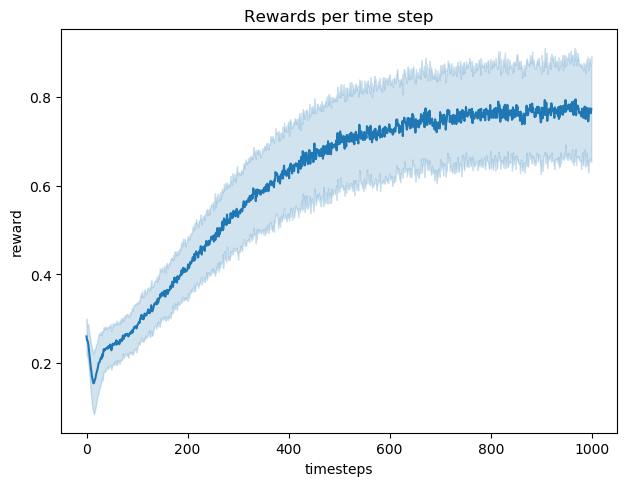
\includegraphics[width=0.28\textwidth]{plots/NAC_BBtime_step_reward.png}	
		\hspace{4mm}
		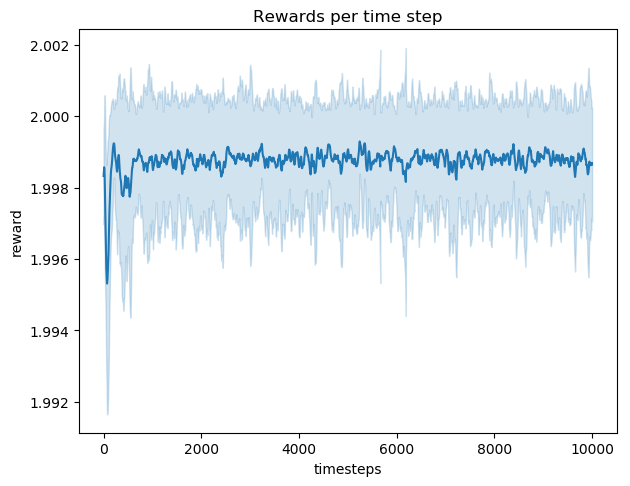
\includegraphics[width=0.285\textwidth]{plots/NAC_CP_time_step_reward.png}
		\hspace{1mm}
		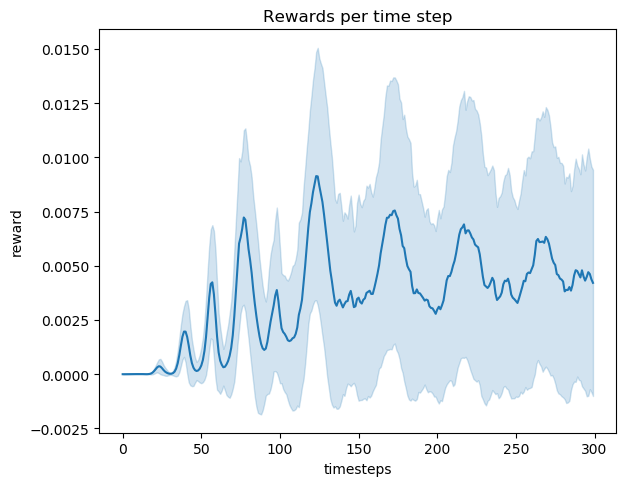
\includegraphics[width=0.3\textwidth]{plots/NAC_Qube_time_step_reward.png}
		\hspace{1.5mm}
		\caption{This figure shows the application of the natural actor critic algorithm on the simulated ball balancer (left column), cart pole (middle column) and qube (right column). The \textit{top row} shows average cumulative trajectory reward for each update during training. The NAC algorithm uses a fixed step size, which means that one update consists of one or more trajectories. The\textit{ bottom row} shows the evaluation of the respective environments, which has been done over 100 trajectories (which may vary in length). The figures show the average reward for each time step and it's standard deviation.}
		\label{fig:nac}
	\end{center}
\end{figure}

\subsection{Evaluation on Qube-v0}

The results we achieved for the Qube were moderate. Our best run had an average cumulative trajectory reward of 0.922. The Qube manages to swing up the pendulum from time to time, but does not hold it in an upright position. We used 500 updates with 4000 steps and a discount factor of 0.99. 

Figure \ref{fig:nac} shows the training of the qube in the top right corner. We can see that a large number of updates is very important for the system. The average cumulative trajectory reward per update still improved during the 500th update. In the bottom right corner of figure \ref{fig:nac}, the average reward per time step can be found. The high standard deviation and the jumpy average illustrate the incapability of the qube to hold the pendulum in an upright position.


% ----- REAL SYSTEM ----- %


\section{Evaluation of Pretrained Models on real systems}

\textbf{Ball Balancer System:} Evaluating our best DDPG model trained in simulation on the real ball balancer was not successful (Figure \ref{fig:rr}, left). The chosen actions were too big and the plate instantly tilted. Additionally, it was not possible for us to reset the environment between the evaluation episodes.

With our best pretrained NAC model, the actions of our policy seemed to strong as well. We tried to execute a model with 10 times smaller actions, but got the same disappointing results.
\\\\
\textbf{Cart Pole System:} Evaluating our best NAC model with nearly perfect rewards on the real cart pole system was not successful (Figure \ref{fig:rr}, right). The actions of the cart had to much power, which is why we clipped the actions from originally [-24, 24] to [-6, 6], but the cart was still far to jumpy to hold the stick upright.

\begin{figure}
	\centering
	
	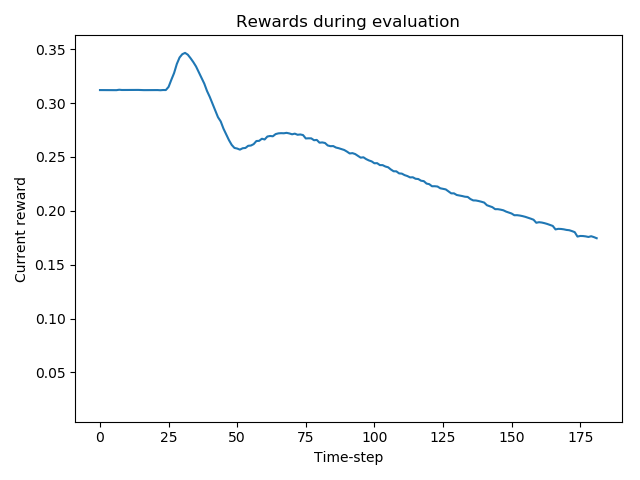
\includegraphics[width=0.35\textwidth]{plots/RR_DDPG_BB_single.png}
	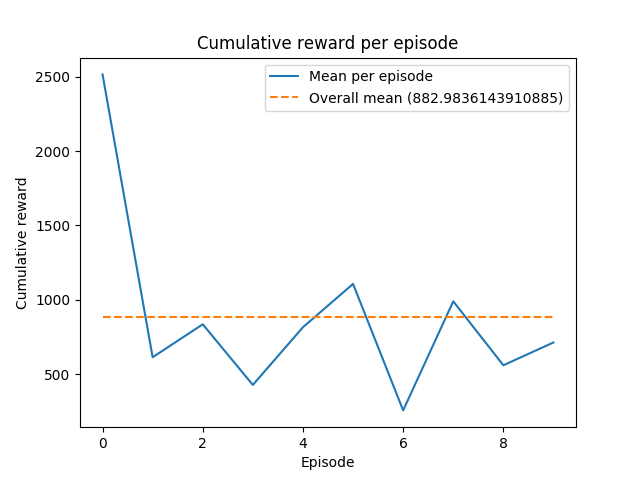
\includegraphics[width=0.37\textwidth]{plots/RR_NAC_CP_10episodes.png}
	
	\caption{On the left side, we can see one episode of DDPG on the real ball balancer system and on the right side, ten episodes of NAC on the real cart pole system. Both algorithms did not perform very well although they run smoothly in simulation.}
	\label{fig:rr}
	
\end{figure}



% ----- DISCUSSION ----- % 

\section{Discussion}
We implemented the DDPG and NAC algorithms and evaluated them on the Quanser Robots environments \textit{BallBalancerSim-v0}, \textit{CartPoleStabShort-v0} and the \textit{Qube-v0}. Both algorithms were able to learn a well performing policy for the first two environments, where the NAC needed less computational time and was more sample efficient. Nonetheless, both algorithms did have troubles to learn a close to optimal policy for the \textit{Qube-v0} environment. They suffered from a very difficult exploration / exploitation trade-off, often with stable learning in the beginning which is overwritten later, or not having enough exploration drive to escape local optima. Further evaluation is needed to optimize the algorithms especially for this environment. Due to technical difficulties it was not really possible to evaluate our pretrained models on the real Quanser Robots systems. Further investigation is needed.
\label{sec:conclusion}






\begin{comment}

We propose several possible extensions and show their performance on a task.\\
Text with citations \cite{RefB} and \cite{RefJ}.
\subsection{Subsection title}
\label{sec:2}
as required. Don't forget to give each section
and subsection a unique label (see Sect.~\ref{sec:1}).
\paragraph{Paragraph headings} Use paragraph headings as needed.
\begin{equation}
a^2+b^2=c^2
\end{equation}

% For one-column wide figures use
\begin{figure}
% Use the relevant command to insert your figure file.
% For example, with the graphicx package use
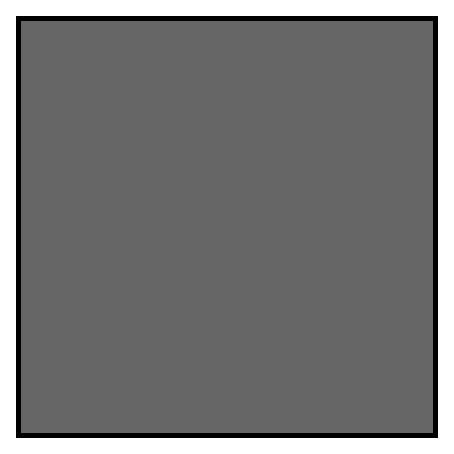
\includegraphics{example.eps}
% figure caption is below the figure
\caption{Please write your figure caption here}
\label{fig:1}       % Give a unique label
\end{figure}
%
% For two-column wide figures use
\begin{figure*}
% Use the relevant command to insert your figure file.
% For example, with the graphicx package use
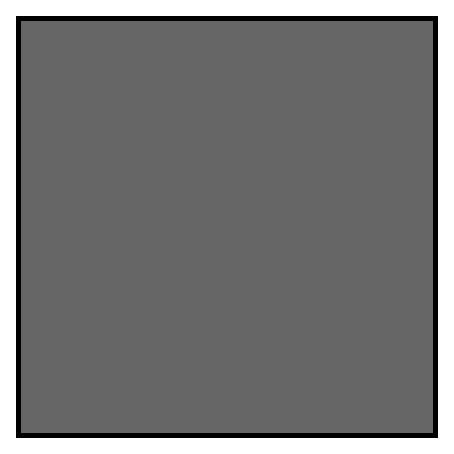
\includegraphics[width=0.75\textwidth]{example.eps}
% figure caption is below the figure
\caption{Please write your figure caption here}
\label{fig:2}       % Give a unique label
\end{figure*}


%
% For tables use
\begin{table}
% table caption is above the table
\caption{Please write your table caption here}
\label{tab:1}       % Give a unique label
% For LaTeX tables use
\begin{tabular}{lll}
\hline\noalign{\smallskip}
first & second & third  \\
\noalign{\smallskip}\hline\noalign{\smallskip}
number & number & number \\
number & number & number \\
\noalign{\smallskip}\hline
\end{tabular}
\end{table}


\end{comment}
%\begin{acknowledgements}
%If you'd like to thank anyone, place your comments here
%and remove the percent signs.
%\end{acknowledgements}

% BibTeX users please use one of
\bibliographystyle{spbasic}      % basic style, author-year citations
%\bibliographystyle{spmpsci}      % mathematics and physical sciences
%\bibliographystyle{spphys}       % APS-like style for physics
\bibliography{project_report.bib}   % name your BibTeX data base

% Non-BibTeX users please use
\begin{comment}


\begin{thebibliography}{}
%
% and use \bibitem to create references. Consult the Instructions
% for authors for reference list style.
%
\bibitem{RefJ}
% Format for Journal Reference
Author, Article title, Journal, Volume, page numbers (year)
% Format for books
\bibitem{RefB}
Author, Book title, page numbers. Publisher, place (year)
% etc

\end{thebibliography}
\end{comment}
\end{document}
% end of file template.tex
